\chapter{Labyrinths}

\section{A maze as a tree}
Let's apply tree navigation techniques to an old problem
of finding path in a maze. For the beginning we'll be assuming that
maze is known (we have full description of a maze before we start).
Here is a simple maze:

\begin{labyrinth}{3}{4}
        \h -++
\v ++-- \h ---
\v ++++ \h --+
\v +--+ \h +++
\end{labyrinth}
%\begin{labyrinth}{3}{4}
%        \h -++
%\v +-+- \h ---
%\v ++++ \h ---
%\v +--+ \h +++
%\labyrinthsolution(0,1){uurddl}
%\end{labyrinth}

Our goal is to find a path in the maze from \textbf{A} to \textbf{B}:

\begin{labyrinth}{3}{4}
        \h -++
\v ++-- \h ---
\v ++++ \h --+
\v +--+ \h +++
\putsymbol(0,4){\small{A}}
\putsymbol(3,3){\small{B}}
\end{labyrinth}

The first question we need to answer is about the maze description.
The answer comes from the following observation: every time we
make a decision navigating the maze we make it from a finite set
of choices:

\begin{labyrinth}{3}{4}
        \h -++
\v ++-- \h ---
\v ++++ \h --+
\v +--+ \h +++
\putsymbol(0,4){\small{A}}
\putsymbol(3,3){\small{B}}
\putsymbol(0,3){\small{1}}
\putsymbol(1,3){\small{2}}
\putsymbol(2,3){\small{3}}
\putsymbol(0,2){\small{4}}
\putsymbol(1,2){\small{5}}
\putsymbol(2,2){\small{6}}
\putsymbol(0,1){\small{7}}
\putsymbol(1,1){\small{8}}
\putsymbol(2,1){\small{9}}
\end{labyrinth}


When we are in location \textbf{7} we can move to location 
\textbf{8}, when in \textbf{8} we can move to \textbf{5} or \textbf{9}.
Let's enumerate all locations and list all possible moves:

$$A\rightarrow 1,\ 1\rightarrow 4,\ 
4\rightarrow 7,\ 7\rightarrow 8,\ 8\rightarrow 5\ or\ 9,
5\rightarrow 2,\ 2\rightarrow 3,\ 3\rightarrow 6\ or\ B.$$

This structure is known from the previous chapter. It's a tree:

\begin{figure}[H]
\centering
\Tree[ .\textbf{A} [ .1 [ .4 [ .7 [ .8 [ [ .5 
[ .2 [ .3 [ 6 \textbf{B} ] ] ] ] 9 ] ] ] ] ] ] 
\end{figure}

\begin{tcolorbox}
\textbf{Assignments:}
describe this tree in Python and print the path from A to B.
\end{tcolorbox}

\section{Maze descriptions}

\begin{tcolorbox}
\textbf{Python:}
You need to learn file I/O, string processing, 
and list comprehensions in Python
\end{tcolorbox}

The maze from the figure above is small and it's easy to describe it by
manually tracing all possible moves.
For bigger mazes we need an automated way of extracting trees
from schematic representations.
For the maze above this can be something like this:

\begin{lstlisting}[language=bash]
0100000
0101111
0101010
0101000
0111110
0000000
\end{lstlisting}

Zeros represent walls and ones represent paths. You may find that the
size -- number of elements -- is different. This is the cost of introducing
walls -- they have a size on the scheme. Extracting a maze from an
image file (scanned or drawn) is technically possible, but difficult.

You can define the scheme of a maze inside your Python program, but
more flexible approach is to save schemas as text files and have one
program that can work with different mazes. 
The following piece of code combines reading the file, splitting it into lines and processing lines
element by element:

\begin{lstlisting}[language=Python,style=codelst2,caption={Python: reading a maze description}]
import sys

f = open(sys.argv[1],"r")
maze = [[x=="1" for x in line] \
       for line in f.read().split("\n") \
       if len(line)>0]
f.close()

print maze
\end{lstlisting}

\section{Converting a maze to a tree. Graphs.}

Now we have a geometrical description
of a maze -- for each element we can tell if it's a path or a wall.
Let's now convert it into a tree representing a node and its children,
or in the case of maze -- an element of a path and
elements of a path on the right-left-top-bottom (if they exist).

To make the work with a maze descriptions more convenient we need to
change the way we are identifying elements of a maze. Before we
used simple enumeration -- for small 3x3 maze above we enumerated all
9 elements from 1 to 9. For a bigger maze enumeration doesn't give a
clear picture -- where, for example, is the element 134 in the 18x13 maze?
 Instead of enumeration we'll be using two numbers -- index of a line
and index of an element position in a line. Element 1 in this notation
becomes (0,0), element 8 -- (2,1). Note zero-based indices -- we'll be
following Python list indexing convention. Enumeration can be easily
restored if needed: for a position $(i,j)$ the "old" 
index is $N\cdot i+j+1$,
where $N$ is the width of a maze: $1=3*0+0+1,\ 8=3*2+1+1$.

The use of enumeration or index pairs makes tree definition 
a little simpler --
each index is unique and we don't need to preserve a path to a node to
distinguish nodes with identical names. A tree can be defined using a
dictionary mapping unique name of a node to a list of children.

The next step is to go over the maze and create the tree. We'll be
going over the maze and for each path element analyze 
surrounding elements --
for element $(i,j)$ we'll need to check elements
$(i-1,j),\ (i+1,j),\ (i,j-1), (i,j+1)$. Adding or subtracting 1
from an index may give new index outside the maze. We'll be
skipping such cases and first write function that returns True
if an index is inside the maze, and False if it's outside:

\begin{lstlisting}[language=Python,style=codelst2,caption={Python: checking index position}]
def is_inside(index,maze_width,maze_hight):
    # checking first index component
    if index[0] < 0 or index[0] >= maze_hight: return False
    # checking second index component
    if index[1] < 0 or index[1] >= maze_width: return False
    # in all other cases index is inside
    return True
\end{lstlisting}

Now we can code the loop over all elements:
\begin{lstlisting}[language=Python,style=codelst,caption={Python: creating tree from maze}]
def create_tree(maze):
    # height of the maze is the number of lines 
    # in the definition
    height = len(maze)
    # we are assuming all lines in the definition 
    # are of the same length
    width = len(maze[0])
    # we are creating empty dictionary ...
    tree = {}
    # ... and first populate it with path elements 
    # mapped to empty lists
    for i in range(height):
        for j in range(width):
            if maze[i][j]: tree[(i,j)] = []
    # now for all elements of the tree we populated
    # lists with indices of surrounding path elements:
    for e in tree:
        i,j = e[0], e[1]
        if is_inside((i-1,j),width,height): 
            if maze[i-1][j]: tree[e].append((i-1,j))
        if is_inside((i+1,j),width,height): 
            if maze[i+1][j]: tree[e].append((i+1,j))
        if is_inside((i,j-1),width,height): 
            if maze[i][j-1]: tree[e].append((i,j-1))
        if is_inside((i,j+1),width,height): 
            if maze[i][j+1]: tree[e].append((i,j+1))
    return tree

\end{lstlisting}

\begin{tcolorbox}
\textbf{Assignment:}
Combine reading a maze from a file, maze parsing,
index verification, and tree creation into one program.
Run the program and review results.
\end{tcolorbox}

As we can see the tree constructed above is different from
trees we've seen before. Note that a node contains its parent
in the list of children -- we do not distinguish
parents and children and operate only with neighbors.
This creates the following problem: the tree navigation
algorithm we used before includes the loop over all
children. If parent node in in the list of children
the loop becomes infinite, or, taking into account
that we used recursion, recursion becomes infinite.

Similar problem arises when a maze has loops.
As a result we may start going into circles:

\begin{labyrinth}{3}{4}
        \h -++
\v +-+- \h ---
\v ++++ \h ---
\v +--+ \h +++
\labyrinthsolution(0,1){uurddl}
\end{labyrinth}

The node structure doesn't form a tree. 
The structure where nodes can form loops is
called a \textbf{graph}. Tree is a graph without loops.

To navigate a graph and find a path between two nodes we
have to modify the algorithm by keeping a record of visited
nodes. Updated version of Depth First Search:

\begin{lstlisting}[language=Python,style=codelst2,caption={Python: DFS with saving visited nodes}]
def DFS(graph,node,visited):
    # adding new node to the list of visited
    visited.append(node)
    # for each node ...
    for child in graph[node]:
    # ... if it's not visitied
        if child not in visited:
            DFS(graph,child,visited)
\end{lstlisting}

Function now takes two more parameters: current node and the list
of visited nodes. When calling the function we are using
an entrance node and empty list.

\begin{tcolorbox}
\textbf{Assignment:}
Combine tree created from a maze definition with DFS function and
print all visited nodes. Use (0,1) as the entrance node.
\end{tcolorbox}

\section{Finding the exit}

We may see that \textbf{DFS} function actually doesn't do any search --
it goes over \textbf{all} nodes. That's not what we need -- the search must
stop when we come to the exit. We have to add new parameter -- \textbf{goal}
that identifies the exit node, and to check each node:

\begin{lstlisting}[language=Python,style=codelst2,caption={Python: DFS with checking the goal}]
def DFS(graph,node,visited,goal):
    visited.append(node)
    # stop if we've reached the goal
    if node == goal: return True
    for child in graph[node]:
        if child not in visited:
            # mini-assignment: why do we need this check?
            if DFS(graph,child,visitedi,goal): return True
    # we'll come here if the maze doesn't have a solution
    return False
\end{lstlisting}


\begin{tcolorbox}
\textbf{Assignment:}
Modify the code of the previous assignment and find the path from
entrance to exit.
\end{tcolorbox}


\section{Breadth first search (BFS)}

When we started talking about navigating a tree we've mentioned
two algorithms. One -- depth first search -- we've learned in
previous sections. Let's consider the second one -- breadth first
search where we go layer by layer in a tree. For general graph
BFS first examines all neighbors (children) of a node before
increasing the depth. Similar to DFS BFS is keeping track of
visited nodes to avoid going into a loop.

The algorithm includes the following steps:

\begin{enumerate}
\item For each node we need to keep path from the start.
\item We create a list \textbf{Q} that for each node we need to check
will keep a queue of pairs (path,node). In the beginning the list contains
only starting node.
\item We create an empty list \textbf{V} to keep visited nodes.
\item The main loop continues while we have nodes to visit, or
in other words -- while the queue \textbf{Q} is not empty.
\item On each step we take first element of \textbf{Q} as our
current node and remove it from the queue.
\item We stop if the current node is our goal.
\item We skip the current node if it's in \textbf{V}.
\item In all other cases we append current node to \textbf{V} and
path and all neighbors of the current node to \textbf{Q}.
\item We continue the main loop.
\end{enumerate}

Here is Python code:

\begin{lstlisting}[language=Python,style=codelst,caption={Python: Breadth first search}]
def BFS(graph,start,goal):
    # initializing queue
    Q = [([start],start)]
    # initalaizing list of visited nodes
    V = []
    # main loop while Q is not empty
    while len(Q)>0:
        path, current_node = Q[0]
        # remove current node from the queue
        Q = Q[1:]
        # are we done?
        if current_node == goal: return (path,True)
        # have we already been here?
        if current_node in V: continue
        # saving current node
        V.append(current_node)
        # loop over all neighbors
        for neighbor in graph[current_node]:
            Q.append((path+[neighbor],neighbor))
    # we cannot reach the goal: returning empty path
    return ([],False)
\end{lstlisting}

You can rewrite the code using more efficient Python structure \textbf{dqueue}.

\begin{tcolorbox}
\textbf{Assignments:}
\begin{enumerate}
\item compare DFS and BFS for the following maze:
\begin{labyrinth}{3}{4}
        \h -++
\v +--- \h ---
\v ++++ \h ---
\v +-++ \h +++
\end{labyrinth}
\item compare DFS and BFS for bigger maze:

\begin{lstlisting}[language=bash]
010000000000
011111111110
010000001000
010111111110
010100000010
010101111110
011100100010
010111101000
010010111110
010110000010
011100111111
000000000000
\end{lstlisting}

Create file with description of the maze, parse it into graph,
do search.
\end{enumerate}
\end{tcolorbox}


\section{Unknown maze}

In previous parts we were assuming that we have a maze
description before we start searching. Our approach
was to create a full graph and use BFS of DFS to
find exit. What if we don't have full maze description and
all we can do is to analyze environment and distinguish
walls and paths -- we can enter a maze, look around
and list all possible moves. We can count our steps
to use (i,j) indices for elements of the maze.

For the simple maze we considered
in the beginning we don't know anything about elements
with question marks -- we know our current position (0,0)
and we see that we can move to (1,0) only.

\begin{labyrinth}{3}{4}
        \h -++
\v ++-- \h ---
\v ++++ \h --+
\v +--+ \h +++
\putsymbol(0,3){\raisebox{2pt}{\tiny{0,0}}}
\putsymbol(1,3){\raisebox{2pt}{\tiny{?}}}
\putsymbol(2,3){\raisebox{2pt}{\tiny{?}}}
\putsymbol(0,2){\raisebox{2pt}{\tiny{1,0}}}
\putsymbol(1,2){\raisebox{2pt}{\tiny{?}}}
\putsymbol(2,2){\raisebox{2pt}{\tiny{?}}}
\putsymbol(0,1){\raisebox{2pt}{\tiny{?}}}
\putsymbol(1,1){\raisebox{2pt}{\tiny{?}}}
\putsymbol(2,1){\raisebox{2pt}{\tiny{?}}}
\end{labyrinth}

When we are in (2,1) we remember our path and know that we can 
move to (2,2) and (1,1):

\begin{labyrinth}{3}{4}
        \h -++
\v ++-- \h ---
\v ++++ \h --+
\v +--+ \h +++
\putsymbol(0,3){\raisebox{2pt}{\tiny{0,0}}}
\putsymbol(1,3){\raisebox{2pt}{\tiny{?}}}
\putsymbol(2,3){\raisebox{2pt}{\tiny{?}}}
\putsymbol(0,2){\raisebox{2pt}{\tiny{1,0}}}
\putsymbol(1,2){\raisebox{2pt}{\tiny{1,1}}}
\putsymbol(2,2){\raisebox{2pt}{\tiny{?}}}
\putsymbol(0,1){\raisebox{2pt}{\tiny{2,0}}}
\putsymbol(1,1){\raisebox{2pt}{\tiny{2,1}}}
\putsymbol(2,1){\raisebox{2pt}{\tiny{2,2}}}
\end{labyrinth}


Would it be possible for us to find the path? The answer
is yes, we can find the path even if don't have full graph
in the beginning -- we can construct it when navigating the
maze, accumulating the knowledge about the operating environment.
If we look at DFS or BFS we can easily find that we don't
need information about the graph, except for the list of
already visited nodes and the list of neighbors.

Our approach will be to start with empty graph,
query environment (look around),
find neighbors and update the graph with new information.

To query environment we'll need a function that returns
all neighbors for a given (i,j) node. We've already done
this in the function converting a maze description into
a graph, only that function went over all maze elements
and now we need a smaller function for a single element.

\begin{tcolorbox}
Assignments:
\begin{enumerate}
\item Write functions that return neighbors.
\item Adjust BFS and DFS functions to navigate a maze
with unknown in the beginning graph.
\end{enumerate}
\end{tcolorbox}

\section{Loading a maze from an image}

So far we were using small mazes. They gave us some idea
how search algorithms work, but size was not big enough
to compare performance and resulting paths. It's inconvenient
to describe a big maze manually by entering 1s and 0s, so
let's load mazes from images. Here is an example of hand-drawn
maze:

\begin{center}
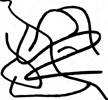
\includegraphics{maze_1s}
\end{center}

You can use a drawing program (PaintBrush or an equivalent),
or draw a maze on paper and then scan or make a picture with
a phone. Make sure lines are thick enough to avoid problems
with image resizing.

You can see an image as a list of pixels going row by row
from the top to the bottom. For a tiny image of 4 rows and
3 columns the first 3 elements of the list (list indices are 0,1,2)
describe the first row, elements with indices 3,4,5 - the second row, etc...

There is a variety of image formats and color modes. Color mode
defines the way to describe color of a pixel. Most popular mode
is RGB (red-green-blue) -- the color is defined as a combination
of three numbers representing red, green, and blue components
of a color. Each number is between 0 and 255. For example:

(0,0,0) -- black

(255,0,0) -- red

(0,255,0) -- green

(0,0,255) -- blue

(255,255,255) -- white

When all RGB components are equal the color is grey: (128,128,128),
(35,35,35), (233,233,233) are all shadows of grey. For
grey-scale images the color may be represented by a single number
between 0 and 255.

We'll not be going into pretty wide area of image processing.
For purposes of the course we need to be able to read the image
into a list of pixels, identify image height and width, 
identify dark pixels
(we'll be considering them as elements of path), change color
of a pixel to indicate found path or visited elements, and save
images into a file.

\begin{tcolorbox}
\textbf{Python:} please refer to Appendix B to learn
basics of image processing.
\end{tcolorbox}

\begin{tcolorbox}
\textbf{Assignments:}
\begin{enumerate}
\item Load maze from an image file, create a graph, find paths
using DFS and BFS.
\item Load maze from an image file, find paths and visited nodes
using both DFS and BFS \footnote{Depending on your system
settings you may get error message when doing recursive search
with DFS -- the number of recursion calls is limited to avoid
infinite recursion. If you see this problem change recursion limit
before calling DFS function: use \textbf{sys.setrecursionlimit(N)}
in Python. Experiment with N - try different values.}
\item Adjust the image file: change color
or visited nodes to green and path nodes to red. Compare results.
\end{enumerate}
\end{tcolorbox}

\section{Adding heuristics - A* search}

Both DFS and BFS can find a path in a maze if it exists.
At the same time their performance (length of the resulting
path and number of visited nodes) may not be satisfactory -- 
sometimes we have to visit all nodes to find the path.
Time and memory requirements can make the search problematic.
Can we improve the search? Given the graph of a maze
(or in more general case -- the graph of our decisions)
we may try to change the way we choose next step. In
previous studies we didn't distinguish between node neighbors --
the order in which we visited them was arbitrary, 
it didn't reflect any idea about a desired order.

Can we change the way we choose the next node to improve
performance (make a path shorter and reduce the number of
visited nodes)? The answer is positive, although the improvement
is not guaranteed -- we can introduce new algorithm that will
work better \textbf{on average}, without improving so called
\textbf{the worst case}. In other words -- it's possible to find
a case when the algorithm doesn't improve performance, but
most of the time it works better.

What would be an "improved" way of choosing next node?
We are in somewhere inside a maze and have several choices.
Intuitively we can choose a node that is closer to the exit than others --
if we know the exit is on the right we may want to move to the
right neighbor node if it's available. More accurately we
need to choose the neighbor so that the number of steps
from the beginning to the node plus our estimation of
the distance from the node to the end is minimal. The method
is called A* (A-Star). Let's try to formalize it.

First we'll need a function that returns our estimation
of the distance from a node to the goal. Given that we can move
up-down-left-right only the distance between two nodes
$(i_1,j_1)$ and $(i_2,j_2)$ can be expressed as a sum of
distances by each direction:

$$ |i_1-i_2| + |j_1-j_2| $$

or as a Python function:
\begin{lstlisting}[language=Python,style=codelst2,caption={Distance between nodes}]
def distance(node1,node2):
    return abs(node1[0]-node2[0]) + abs(node1[1]-node2[1])
\end{lstlisting}

Similar to BFS we'll keep the queue for nodes to visit, but in A*
those nodes have to be sorted based on the measure we discussed above
(number of steps from the beginning plus expected distance).
This functionality can be implemented with basic Python lists,
but more convenient is to use already available modules.
Pythons provides all we need with module \textbf{heapq}. 

Function \textbf{heappush} adds new element to the sorted queue 
preserving the order. For example adding 2 to the list of [1, 3, 4, 5]
creates new list on [1, 2, 3, 4, 5]. If element has several
components \textbf{heappush} the sort order is according to the
first component. 

Function \textbf{heappop} returns first ("smallest") element from
the queue and removes it from queue.

Queue element for A* search has to contain the following components:
\begin{enumerate}
\item number of steps from the beginning plus estimation of the deistance
to the end -- the value we'll be using to sort element (remember --
we want to prioritize nodes with smaller value).
\item number of steps from the beginning
\item path from the beginning
\item node
\end{enumerate}

\begin{lstlisting}[language=Python,style=codelst2,caption={Python: A* search}]
from heapq import heappop
from heapq import heappush

def AStar(graph,start,goal):
    Q = []
    heappush( Q, (distance(start,goal),0,[start],start) )
    V = []
    while len(Q)>0:
        dist, from_start, path, current_node = heappop(Q)
        if current_node == goal: return (path,V,True)
        if current_node in V: continue
        V.append(current_node)
        for neighbor in graph[current_node]:
            dist = distance(neighbor,goal)
            Q.append((from_start+dist,from_start+1,path+[neighbor],neighbor))
    return ([],[],False)
\end{lstlisting}

You may find that the code is pretty similar to the code of BFS.
The differences are in the components of \textbf{Q} discussed before,
and in the use of \textbf{heapq} instead of plain Python lists.

\begin{tcolorbox}
\textbf{Assignments:}
\begin{enumerate}
\item Load maze from an image file, create a graph, find paths
using A*.
\item Adjust the image file: change color
or visited nodes to green and path nodes to red. Compare results 
(paths and visited nodes) with DFS and BFS.
\item Experiment with the distance function -- try to introduce
the distance between nodes in a different way. Compare results.
\end{enumerate}
\end{tcolorbox}

\section{Challenge 1: build library of search functions and maze processing}

\begin{tcolorbox}
\textbf{Python:} please refer to Appendix to learn
module programming -- file organization and module function access.
\end{tcolorbox}

By this time you have already developed several useful functions:
\begin{enumerate}
\item Search functions: DFS, BFS, A*.
\item Maze operations: loading from a maze description, loading from an image file.
\item Creating a graph from a maze description.
\end{enumerate}

The first challenge in this course is to create Python module providing
this functionality. Keep search and maze-related functions separately.

After you are done with writing module redo your assignments using
the module. The goal is learn how to write reusable code.






